\documentclass[11pt]{article}
\usepackage{amsmath,amsbsy,amssymb,verbatim,fullpage,ifthen,graphicx,bm,amsfonts,amsthm,url}
\usepackage{graphicx}
\usepackage{xcolor}
\newcommand{\mfile}[1]  {{\small \verbatiminput{./#1}}} % Jeff Fessler, input matlab file
\newcommand{\tmop}[1]{\ensuremath{\operatorname{#1}}}
\newcommand{\R}{\mathbb{R}}
\newcommand{\C}{\mathbb{C}}
\newcommand{\Z}{\mathbb{Z}}
\newcommand{\A}{\mathcal{A}}
\newcommand{\minimize}{\operatorname*{minimize\ }}
\newcommand{\maximize}{\operatorname*{maximize}}
\newcommand{\opdet}[1]{\operatorname{\textbf{det}}\left(#1\right)}
\newcommand{\optr}[1]{\operatorname{\textbf{tr}}\left(#1\right)}
\newcommand{\answer}[2][blue]{\ifdefined\AnswerDefine{\color{#1}\it#2}\fi}
\newcommand{\mtx}[1]{\mathbf{#1}}
\newcommand{\vct}[1]{\mathbf{#1}}
\def \lg       {\langle}
\def \rg       {\rangle}
\def \mA {\mtx{A}}
\def \mI {\mtx{I}}
\def \mJ {\mtx{J}}
\def \mU {\mtx{U}}
\def \mS {\mtx{S}}
\def \mV {\mtx{V}}
\def \mW {\mtx{W}}
\def \mLambda {\mtx{\Lambda}}
\def \mSigma {\mtx{\Sigma}}
\def \mX {\mtx{X}}
\def \mY {\mtx{Y}}
\def \mZ {\mtx{Z}}
\def \zero     {\mathbf{0}}
\def \vzero    {\vct{0}}
\def \vone    {\vct{1}}
\def \vu {\vct{u}}
\def \vv {\vct{v}}
\def \vx {\vct{x}}
\def \vy {\vct{y}}
\def \vz {\vct{z}}
\def \vphi {\vct{\phi}}
\def \vmu {\vct{\mu}}
\def \R {\mathbb{R}}


\usepackage{xspace}
\makeatletter
\DeclareRobustCommand\onedot{\futurelet\@let@token\@onedot}
\def\@onedot{\ifx\@let@token.\else.\null\fi\xspace}

\def\eg{\emph{e.g}\onedot} \def\Eg{\emph{E.g}\onedot}
\def\ie{\emph{i.e}\onedot} \def\Ie{\emph{I.e}\onedot}
\def\cf{\emph{c.f}\onedot} \def\Cf{\emph{C.f}\onedot}
\def\etc{\emph{etc}\onedot} \def\vs{\emph{vs}\onedot}
\def\wrt{w.r.t\onedot} \def\dof{d.o.f\onedot}
\def\etal{\emph{et al}\onedot} \def\st{\emph{s.t}\onedot}
\pagestyle{plain}
\usepackage{listings}
\usepackage{color} %red, green, blue, yellow, cyan, magenta, black, white
\definecolor{mygreen}{RGB}{28,172,0} % color values Red, Green, Blue
\definecolor{mylilas}{RGB}{170,55,241}
\lstset{language=Matlab,%
    %basicstyle=\color{red},
    breaklines=true,%
    morekeywords={matlab2tikz},
    keywordstyle=\color{blue},%
    morekeywords=[2]{1}, keywordstyle=[2]{\color{black}},
    identifierstyle=\color{black},%
    stringstyle=\color{mylilas},
    commentstyle=\color{mygreen},%
    showstringspaces=false,%without this there will be a symbol in the places where there is a space
    numbers=left,%
    numberstyle={\tiny \color{black}},% size of the numbers
    numbersep=9pt, % this defines how far the numbers are from the text
    emph=[1]{for,end,break},emphstyle=[1]\color{red}, %some words to emphasise
    %emph=[2]{word1,word2}, emphstyle=[2]{style},    
}

\title{{\bf Homework Set 2, CPSC 8420, Spring 2022}} % Change to the appropriate homework number
\author{\Large\underline{William Sherrer}}
\date{\textbf{\Large\textcolor{red}{Due 03/17/2022, Thursday, 11:59PM EST}}} % put your name in the LastName, FirstName format
%\date{\today}

\begin{document}
	\maketitle
	

	\section*{Problem 1}
	For PCA, from the perspective of maximizing variance, please show that the solution of $\bm{\phi}$ to $\maximize \|\mX \bm{\phi}\|^2_2, \st \ \|\bm{\phi}\|_2=1$ is exactly the first column of $\mU$, where $[\mU,\mS]=svd(\mX^T\mX)$. (Note: you need prove why it is optimal than any other reasonable combinations of $\mU_i$, say $\hat{\bm{\phi}}=0.8*\mU(:,1)+0.6*\mU(:,2)$ which also  satisfies $\|\hat{\bm{\phi}}\|_2=1$.)\\
	
	
We say that this is equivalent to $\max tr(\phi^T X^T X \phi)$. If we compute $[\mU,\mS, \mV]=svd(\mX^T\mX)$, then we have $\phi_1 = U(:, 1)$, and the variance $\| X \phi \|^2 = S^2(1,1)$. Using svd we can compute that $U \Sigma U^T = X^T X => \sum{\lambda_i u_i u^T_i}$. We start by letting $\phi_1 = U_1$. Therefore $\phi^T X^T X \phi$ can be rewritten as $U_1^T \Sigma \lambda_i u_i u^T_i U_1$ and since all of the columns of U are orthogonal to each other the equation will collapse  to $= \lambda_1$.\\\\

Let's say that $X^TXv_1 = \lambda_1 v_1$. To find  we multiply by $X$ to get $X* X^TXv_1 = \lambda_1 X v_1$ and then further simplifying $XX^T = \lambda_1$. Therefore we can conclude that the corresponding eigenvalue is exactly equal to the variance of the data set.\\

The end result is that the first $k$ principal components of $X$ correspond exactly to the eigenvectors of the covariance matrix S ordered by their eigenvalues. Moreover, the eigenvalues are exactly equal to the variance of the dataset along the corresponding eigenvectors. Therefore we satisfy $\phi_1 = U(:, 1)$, and the variance $\| X \phi \|^2 = S^2(1,1)$. This is optimal as $\hat{\phi} = \Sigma a_i u_i$ with $a_i$ being a scalar. Since the magnitude $\|a\| = 1$ we can say that $\|\hat{\phi}\| = 1$
	
	\section*{Problem 2}
	Why might we prefer to minimize the sum of absolute residuals instead of the residual sum of squares for some data sets? Recall clustering method $K$-means when calculating the centroid, it is to take the mean value of the data-points belonging to the same cluster, so what about $K$-medians? What is its advantage over of $K$-means? Please use a synthetic (toy) experiment to illustrate your conclusion.\\\\
	
Sum of absolute residuals is more resilient to outliers in a data set than sum of squares. In the sum of squares, the distances from the mean are squared, so large deviations are weighted more heavily, and thus outliers can heavily influence it. In the sum of absolutes, the deviations of a small number of outliers are irrelevant. It is also more useful in data set where there isn't a clear mean or variance.\\\\

Similar to the same problem with mean for number sets, $K$-means can be prone to falling for outliers. The $K$-means algorithm shift the centroid to the mean vector of the cluster, whilst $K$-medians shifts to the median vector of the vector. If there are several outliers present in the dataset, this could vastly effect $K$-means in where it shifts it centroids.\\\\
Figure 1: Centroid position of data with and without outliers.\\
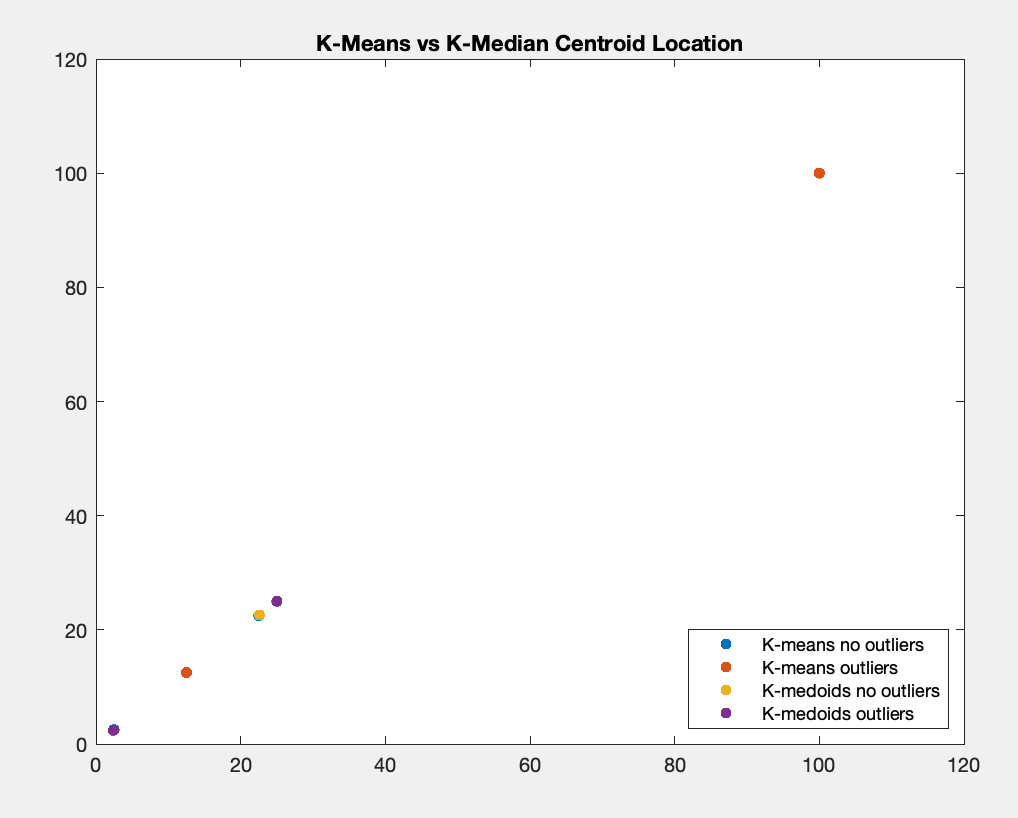
\includegraphics[scale=.6]{kmeans_vs_kmedians}\\
Some of the centroid points are not visible because they are in the same location as other centroid positions.\\\\
	
	
	\section*{Problem 3}
	Let's revisit Least Squares Problem: $\minimize \limits_{\bm{\beta}} \frac{1}{2}\|\vy-\mA\bm{\beta}\|^2_2$, where $\mA\in\R^{n\times p}$.
	\begin{enumerate}
		\item Please show that if $p>n$, then vanilla solution $(\mA^T\mA)^{-1}\mA^T\vy$ is not applicable any more.	\\
		Least squares is applicable when  a matrix has a set of linear equations. (more equations than unknowns). Since $y$ is a linear combination of $A$, we assume that the columns of $A$ are linearly independent, however, this is not the case when $p > n$ therefore the vanilla solution does not apply. 
		\item Let's assume $\mA=[1, 2, 4;1, 3, 5; 1, 7, 7; 1, 8, 9], \vy=[1;2;3;4]$. Please show via experiment results that Gradient Descent method will obtain the optimal solution with  Linear Convergence rate if the learning rate is fixed to be $\frac{1}{\sigma_{max}(\mA^T\mA)}$, and $\bm{\beta}_0=[0;0;0]$.	
		
Figure 2: The Loss will eventually converge as we increase \# of iterations\\
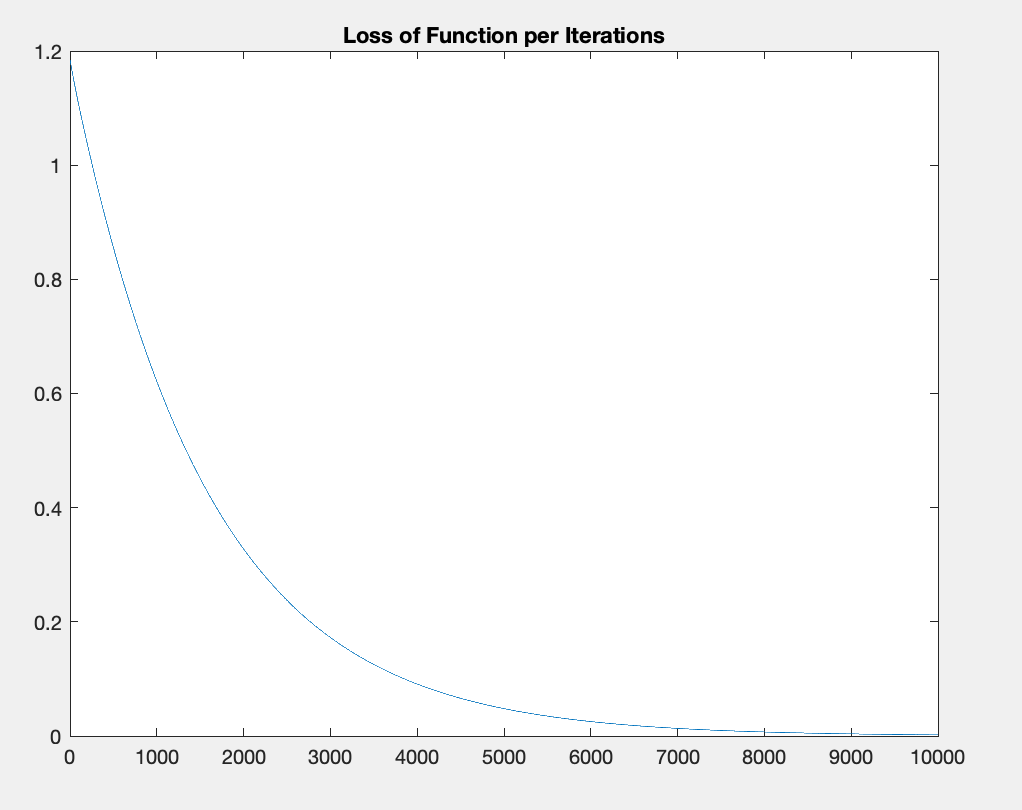
\includegraphics[scale=.6]{Loss_least_squares}

 
		\item Now let's consider ridge regression: $\minimize \limits_{\bm{\beta}} \frac{1}{2}\|\vy-\mA\bm{\beta}\|^2_2+\frac{\lambda}{2} \|\bm{\beta}\|^2_2$, where  $\mA,\vy,\bm{\beta}_0$ remains the same as above while learning rate is fixed to be $\frac{1}{\lambda+\sigma_{max}(\mA^T\mA)}$ where $\lambda$ varies from $0.1,1,10,100,200$, please show that Gradient Descent method with larger $\lambda$ converges faster. \\

Figure 3: Loss of function per lambda\\
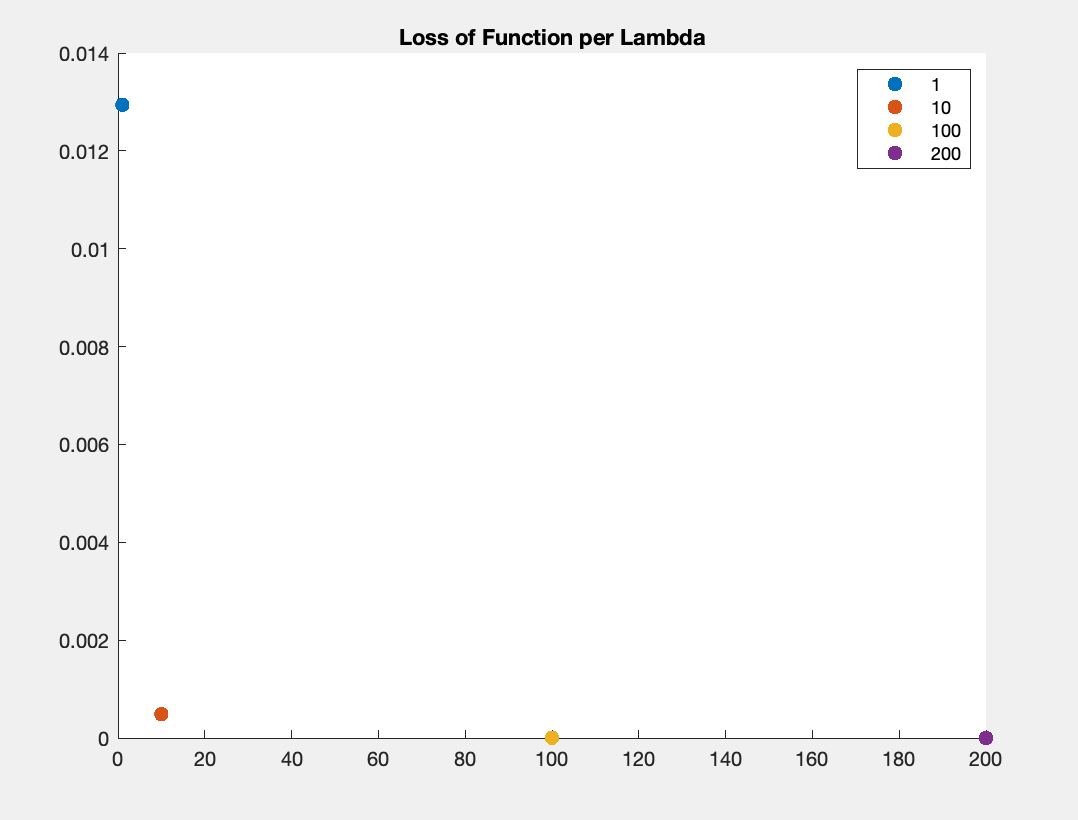
\includegraphics[scale=.55]{Loss_ridge}
\end{enumerate}


	
	\section*{Problem 4}
	Please download the image from \url{https://en.wikipedia.org/wiki/Lenna#/media/File:Lenna_(test_image).png} with dimension $512\times512\times3$. Assume for each RGB channel data $X$, we have $[U,\Sigma,V]=svd(X)$. Please show each compression ratio and reconstruction image if we choose first $2, 5, 20, 50,80,100$ components respectively. Also please determine the best component number to obtain a good trade-off between data compression ratio and reconstruction image quality. (Open question, that is your solution will be accepted as long as it's reasonable.)\\\\
I personally believe that the 80 columns is a good tradeoff between compression ratio and image quality. The data showed is roughly 16\% of the original image however when viewed at a reasonable distance it still looks very comparable to the original image.
\begin{figure}[!h]
	\centering
	\caption{Compression ratio = $\frac{2}{512} = 0.004$}
	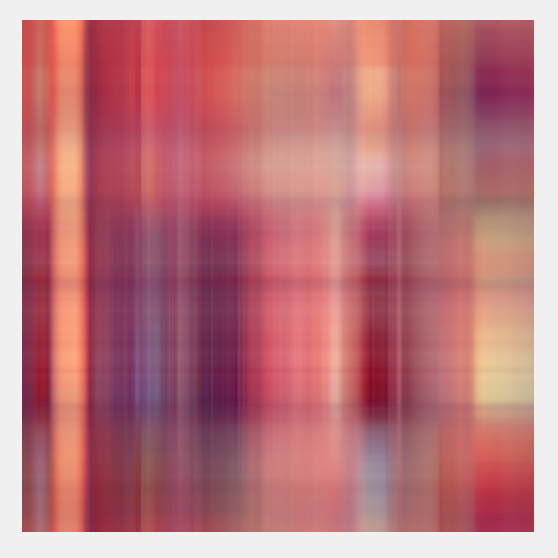
\includegraphics[scale=.6]{lenna_2}
\end{figure}

\begin{figure}[!h]
\centering
	\caption{Compression ratio = $\frac{5}{512} = 0.01$}
	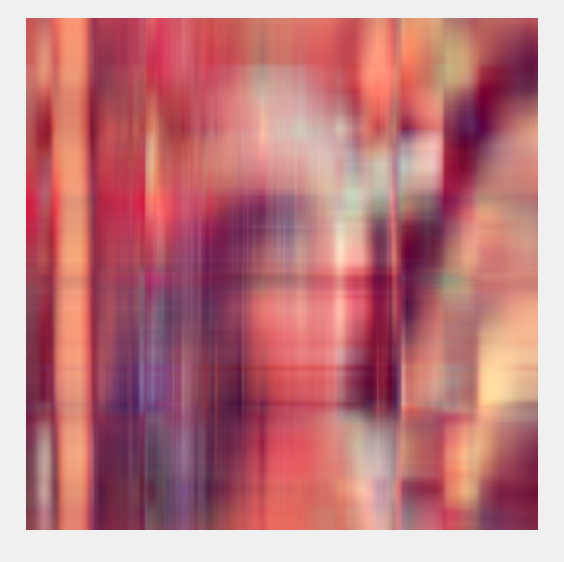
\includegraphics[scale=.6]{lenna_5}
\end{figure}

\begin{figure}[!h]
\centering
	\caption{Compression ratio = $\frac{20}{512} = 0.04$}
	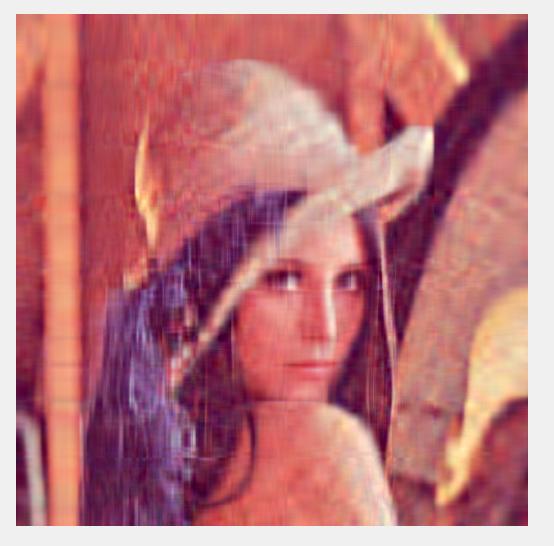
\includegraphics[scale=.6]{lenna_20}
\end{figure}

\begin{figure}[!h]
\centering
	\caption{Compression ratio = $\frac{50}{512} = 0.097$}
	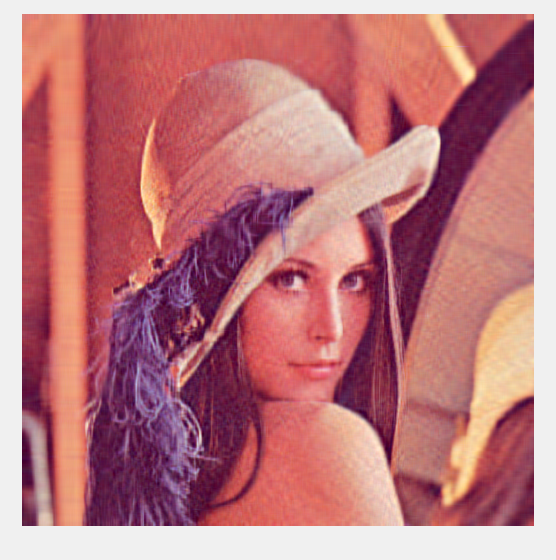
\includegraphics[scale=.6]{lenna_50}
\end{figure}

\begin{figure}[!h]
\centering
	\caption{Compression ratio = $\frac{80}{512} = 0.156$}
	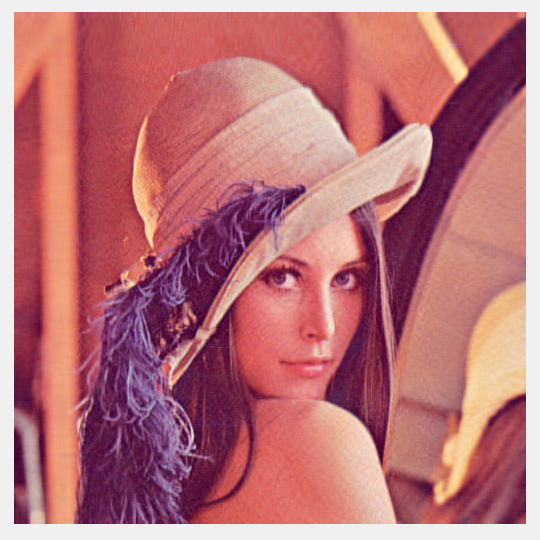
\includegraphics[scale=.6]{lenna_80}
\end{figure}

\begin{figure}[!h]
\centering
	\caption{Compression ratio = $\frac{100}{512} = 0.195$}
	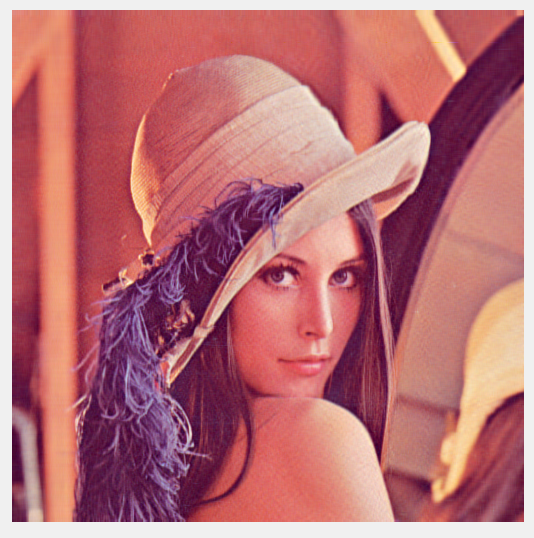
\includegraphics[scale=.6]{lenna_100}
\end{figure}

\section*{Code for homework}
Kmeans vs Kmedians toy experiment
\lstinputlisting{kmeans_vs_kmedians.m}
Gradient Descent using Vanilla Least Squares
\lstinputlisting{grad_descent_vanilla.m}
Gradient Calculation for Least Squares
\lstinputlisting{gradient_least.m}
Gradient Descent using Ridge Regression
\lstinputlisting{grad_descent_ridge.m}
Gradient Calculation for Ridge Regression
\lstinputlisting{gradient_ridge.m}
\end{document}
